\documentclass[UTF8,aspectratio=169,10pt]{ctexbeamer}

% ---- 主题与配色 ----
\usetheme{Madrid}
\usecolortheme{default}
\usefonttheme{professionalfonts}

% ---- 包 ----
\usepackage{amsmath,amssymb,bm}
\usepackage{graphicx}
\usepackage{booktabs}
\usepackage{tikz}
\usetikzlibrary{positioning,calc}
\usepackage{xcolor}
\usepackage{newtxmath}        % Times 风格数学字体
\usepackage{fontspec}

% ---- 正文字体 ----
\setmainfont{Times New Roman}
\setsansfont{Arial}
\setmonofont{Consolas}
\setCJKmainfont{SimSun}

% ---- 图片搜索路径 ----
\graphicspath{
  {../assets/}
  {../assets/q3_visualization/}
  {../assets/q3_comparison/}
  {../assets/q3_fem/}
}

% ---- 自定义颜色 ----
\definecolor{tjublue}{RGB}{0,74,132}
\definecolor{tjuaccent}{RGB}{180,58,72}
\definecolor{softgray}{RGB}{245,247,250}
\definecolor{darkbg}{RGB}{15,30,50}

% ---- Beamer 颜色 ----
\setbeamercolor{palette primary}{bg=tjublue,fg=white}
\setbeamercolor{palette secondary}{bg=tjublue!85,fg=white}
\setbeamercolor{palette tertiary}{bg=tjublue!70,fg=white}
\setbeamercolor{frametitle}{bg=tjublue,fg=white}
\setbeamercolor{title}{fg=tjublue}
\setbeamercolor{block title}{bg=tjublue,fg=white}
\setbeamercolor{block body}{bg=softgray,fg=black}
\setbeamercolor{alerted text}{fg=tjuaccent}

% ---- 导航隐藏 ----
\setbeamertemplate{navigation symbols}{}
\setbeamertemplate{caption}[numbered]

% ---- 辅助命令 ----
\newcommand{\keypoint}[1]{\begin{block}{要点}#1\end{block}}
\newcommand{\highlight}[1]{\textcolor{tjuaccent}{#1}}

% ====== 标题信息 ======
\title[结构动力学 Q3]{带集中质量与局部弹簧支承\\Euler--Bernoulli 梁自由振动的\\解析解与有限元验证}
\author{王子传 \quad 吕天翔 \quad 方思哲}
\institute{天津大学机械工程学院}
\date{}

\begin{document}

% ====== 1. 封面 ======
\begin{frame}
  \vspace{0.5em}
  \begin{beamercolorbox}[wd=\linewidth,rounded=true,shadow=true,sep=1.2em,center]{frametitle}
    {\Large\bfseries 带集中质量与局部弹簧支承 Euler--Bernoulli 梁\\[0.3em]自由振动的解析解与有限元验证}
  \end{beamercolorbox}
  \vspace{1.5em}
  \begin{center}
    {\large 王子传 \quad 吕天翔 \quad 方思哲}\\[0.6em]
    天津大学机械工程学院\\[2em]
    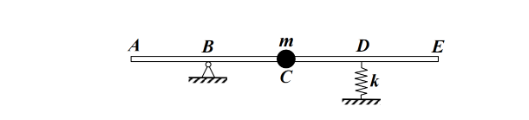
\includegraphics[width=0.50\linewidth]{image-20260616001638017.png}
  \end{center}
\end{frame}

% ====== 2. 汇报提纲 ======
\begin{frame}{汇报内容}
  \begin{columns}[T,onlytextwidth]
    \column{0.55\linewidth}
    \begin{enumerate}
      \item 研究背景与问题描述
      \item 解析解建模与推导
      \item 有限元模型与 Fortran 实现
      \item 解析解与 FEM 结果对比
      \item 结论与展望
    \end{enumerate}
    \column{0.40\linewidth}
    \begin{block}{技术路线}
      \[
      \text{问题建模}\longrightarrow
      \text{解析求解}\longrightarrow
      \text{数值验证}
      \]
    \end{block}
  \end{columns}
\end{frame}

% ====== 3. 研究背景 ======
\begin{frame}{研究背景}
  \begin{itemize}
    \item 梁结构是机械、土木、航空航天和交通装备中的典型承载构件。
    \item 局部支承、附加质量、弹簧连接等因素会显著改变结构动力特性。
    \item 对含局部离散构件的连续梁，既需要解析建模，也需要数值验证。
  \end{itemize}
  \vspace{1em}
  \begin{block}{核心关注}
    \[
    \text{局部约束 / 集中质量 / 弹簧支承}
    \quad\Longrightarrow\quad
    \text{固有频率、振型、动力响应变化}
    \]
  \end{block}
\end{frame}

% ====== 4. 研究对象 ======
\begin{frame}{结构模型}
  \begin{columns}[T,onlytextwidth]
    \column{0.48\linewidth}
    \begin{itemize}
      \item 均质等截面 Euler--Bernoulli 梁
      \item 总长 $4l$，其中 $AB=BC=CD=DE=l$
      \item $B$ 点：外部铰支座
      \item $C$ 点：附加集中质量 $m$
      \item $D$ 点：竖向线性弹簧 $k$ 与地面连接
      \item 初始时刻 $C$ 点具有横向速度 $v_0$
    \end{itemize}
    \column{0.48\linewidth}
    \centering
    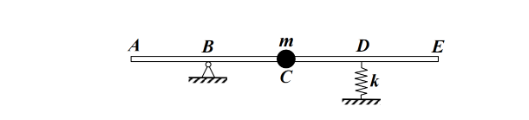
\includegraphics[width=\linewidth]{image-20260616001638017.png}
  \end{columns}
\end{frame}

% ====== 5. 研究目标 ======
\begin{frame}{研究目标}
  \begin{columns}[T,onlytextwidth]
    \column{0.45\linewidth}
    \begin{block}{待求解量}
      \begin{enumerate}
        \item 固有频率 $\omega_n$
        \item 振型函数 $\phi_n(x)$
        \item 初始速度作用下的动力响应 $w(x,t)$
        \item 解析解与有限元解的一致性验证
      \end{enumerate}
    \end{block}
    \column{0.50\linewidth}
    \begin{block}{技术路线}
      \begin{align*}
        &\text{解析传递矩阵法}\\
        {+}\;&\text{Euler--Bernoulli 梁有限元法}\\
        {+}\;&\text{Python 后处理对比}
      \end{align*}
    \end{block}
  \end{columns}
\end{frame}

% ====== 6. 基本假设 ======
\begin{frame}{基本假设}
  \begin{itemize}
    \item 梁满足 Euler--Bernoulli 梁理论。
    \item 材料线弹性，小变形。
    \item 梁为均质等截面。
    \item 集中质量只提供横向惯性。
    \item 弹簧为线性竖向弹簧。
    \item $B$ 点支座只约束竖向位移，不约束转角。
  \end{itemize}
  \vspace{1em}
  \begin{alertblock}{关键说明}
    \[
    B\text{ 点为连续梁上的外部简单支承点，而非梁内铰。}
    \]
  \end{alertblock}
\end{frame}

% ====== 7. 控制方程 ======
\begin{frame}{控制方程}
  \begin{columns}[T,onlytextwidth]
    \column{0.48\linewidth}
    \begin{block}{Euler--Bernoulli 梁段方程}
      设线密度：
      \[
      \mu=\rho S
      \]
      控制方程：
      \[
      EJ\frac{\partial^4 w}{\partial x^4}
      +\rho S\frac{\partial^2 w}{\partial t^2}
      =0
      \]
    \end{block}
    \column{0.48\linewidth}
    \begin{block}{分离变量}
      令：
      \[
      w(x,t)=\phi(x)q(t)
      \]
      空间方程：
      \[
      \phi^{(4)}-\lambda^4\phi=0
      \]
    \end{block}
  \end{columns}
\end{frame}

% ====== 8. 无量纲化 ======
\begin{frame}{无量纲化}
  \begin{columns}[T,onlytextwidth]
    \column{0.40\linewidth}
    \begin{block}{坐标归一化}
      \[
      \xi=\frac{x}{l},\qquad
      \beta=\lambda l
      \]
      节点位置：
      \[
      A:0,\; B:1,\; C:2,\; D:3,\; E:4
      \]
    \end{block}
    \column{0.28\linewidth}
    \begin{block}{空间方程}
      \[
      Y''''-\beta^4Y=0
      \]
    \end{block}
    \column{0.28\linewidth}
    \begin{block}{频率恢复}
      \[
      \omega_n=
      \frac{\beta_n^2}{l^2}
      \sqrt{\frac{EJ}{\rho S}}
      \]
    \end{block}
  \end{columns}
  \vspace{1em}
  求解 $\beta_n$ 是整个解析解的核心——得到 $\beta_n$ 即可恢复实频。
\end{frame}

% ====== 9. 边界条件 ======
\begin{frame}{边界条件}
  \begin{columns}[T,onlytextwidth]
    \column{0.48\linewidth}
    \begin{block}{自由端 $A,\;E$}
      \[
      Y''(0)=Y'''(0)=0
      \]
      \[
      Y''(4)=Y'''(4)=0
      \]
      弯矩与剪力为零。
    \end{block}
    \column{0.48\linewidth}
    \begin{block}{$B$ 点铰支}
      \[
      Y(1)=0
      \]
      $Y,\;Y',\;Y''$ 连续；\\
      $Y'''$ 可因支座反力跳跃。
    \end{block}
  \end{columns}
\end{frame}

% ====== 10. 跳跃条件 ======
\begin{frame}{集中质量与弹簧跳跃条件}
  \begin{columns}[T,onlytextwidth]
    \column{0.48\linewidth}
    \begin{block}{$C$ 点集中质量}
      剪力跳跃与惯性力平衡：
      \[
      \begin{aligned}
      Y'''(2^+)-Y'''(2^-)
      &=\alpha\beta^4Y(2),\\[0.3em]
      \alpha&=\frac{m}{\rho Sl}
      \end{aligned}
      \]
    \end{block}
    \column{0.48\linewidth}
    \begin{block}{$D$ 点竖向弹簧}
      剪力跳跃与弹簧力平衡：
      \[
      \begin{aligned}
      Y'''(3^+)-Y'''(3^-)
      &=-\kappa Y(3),\\[0.3em]
      \kappa&=\frac{kl^3}{EJ}
      \end{aligned}
      \]
    \end{block}
  \end{columns}
\end{frame}

% ====== 11. 传递矩阵法 ======
\begin{frame}{传递矩阵法}
  \begin{block}{状态向量}
    \[
    \mathbf z(\xi)=
    \begin{bmatrix}
    Y & Y' & Y'' & Y'''
    \end{bmatrix}^{T}
    \]
  \end{block}
  \vspace{0.5em}
  \begin{columns}[T,onlytextwidth]
    \column{0.48\linewidth}
    \begin{block}{梁段传递}
      \[
      \mathbf z(\xi+s)=\mathbf P(s)\,\mathbf z(\xi)
      \]
    \end{block}
    \column{0.48\linewidth}
    \begin{block}{跳跃矩阵}
      \[
      \mathbf z(2^+)=\mathbf J_m\,\mathbf z(2^-)
      \]
      \[
      \mathbf z(3^+)=\mathbf J_k\,\mathbf z(3^-)
      \]
    \end{block}
  \end{columns}
\end{frame}

% ====== 12. 频率方程 ======
\begin{frame}{频率方程}
  \begin{columns}[T,onlytextwidth]
    \column{0.48\linewidth}
    \begin{block}{左端自由}
      \[
      \mathbf z(0)=
      \begin{bmatrix}
      a & b & 0 & 0
      \end{bmatrix}^{T}
      \]
    \end{block}
    \begin{block}{未知向量}
      设 $B$ 点剪力跳跃为 $R$：
      \[
      \mathbf c=
      \begin{bmatrix}
      a & b & R
      \end{bmatrix}^{T}
      \]
    \end{block}
    \column{0.48\linewidth}
    \begin{block}{特征方程}
      右端边界条件导出：
      \[
      \mathbf A(\beta)\,\mathbf c=\mathbf 0
      \]
      非平凡解条件：
      \[
      \det\mathbf A(\beta)=0
      \]
      正根 $\beta_n$ 给出无量纲频率 $\bar{\omega}_n=\beta_n^2$。
    \end{block}
  \end{columns}
\end{frame}

% ====== 13. 特征根可视化 ======
\begin{frame}{解析特征根可视化}
  \begin{columns}[T,onlytextwidth]
    \column{0.62\linewidth}
    \centering
    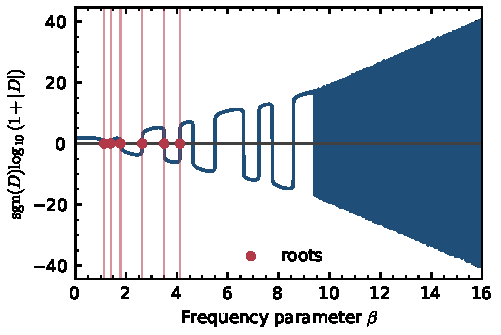
\includegraphics[width=\linewidth]{q3_characteristic_roots.pdf}
    \column{0.34\linewidth}
    \small
    \begin{itemize}
      \item[纵轴] 采用 $\operatorname{sgn}(D)\log_{10}(1+|D|)$ 压缩宽动态范围
      \item[红点] 特征根 $\beta_n$ 位于 $D=0$ 的过零点
      \item[低阶] $\beta_{1\sim4}$ 分布清晰、间距规律
      \item[高阶] $\beta>6$ 后行列式剧烈振荡，根间距收窄
      \item[$\bar\omega_n$] 无量纲频率由 $\beta_n^2$ 恢复
    \end{itemize}
  \end{columns}
\end{frame}

% ====== 14. 解析振型 ======
\begin{frame}{解析振型函数}
  \begin{columns}[T,onlytextwidth]
    \column{0.66\linewidth}
    \centering
    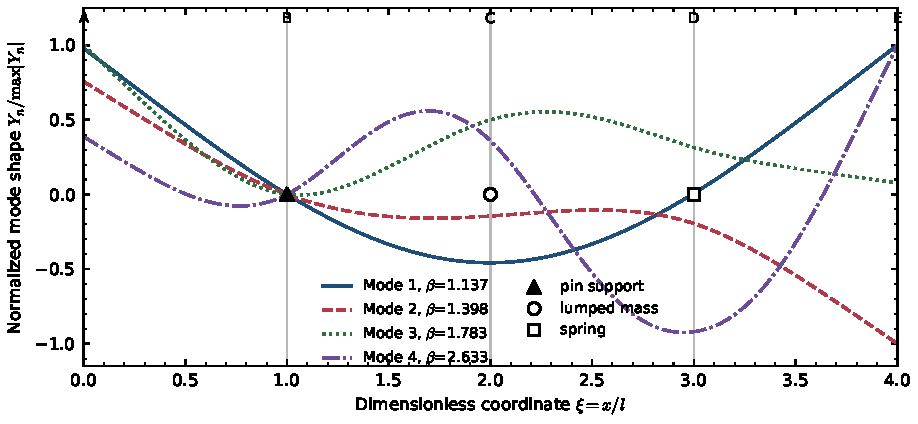
\includegraphics[width=\linewidth]{q3_mode_shapes.pdf}
    \column{0.30\linewidth}
    \small
    \begin{itemize}
      \item 各阶振型均满足 $Y(1)=0$（$B$ 点支承）
      \item Mode 1：半波形态，$C$ 点振幅最大
      \item Mode 2：$B\!-\!C$ 间出现节点，弹簧端接近驻点
      \item Mode 3、4：节线数递增，局部弯曲加剧
      \item $C$ 点（质量）：位移连续，斜率不变
      \item $D$ 点（弹簧）：位移连续，$\phi'$ 有转角
    \end{itemize}
  \end{columns}
\end{frame}

% ====== 15. C点解析响应 ======
\begin{frame}{$C$ 点解析动力响应}
  \begin{columns}[T,onlytextwidth]
    \column{0.42\linewidth}
    \begin{block}{模态响应公式}
      \[
      w(x,t)=
      \sum_{n=1}^{\infty}
      \phi_n(x)\,
      \frac{m v_0\phi_n(2l)}
      {M_n\omega_n}
      \sin\omega_n t
      \]
    \end{block}
    \vspace{0.3em}
    初始速度 $v_0$ 作用于 $C$ 点集中质量，$C$ 点响应最能体现初始激励特征。
    \column{0.54\linewidth}
    \centering
    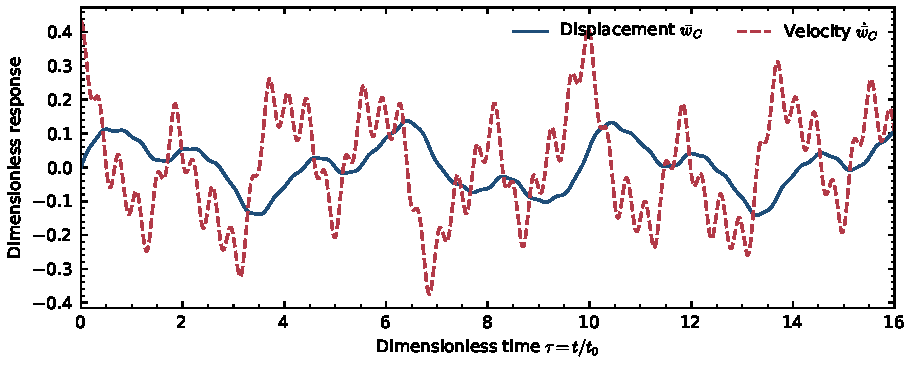
\includegraphics[width=\linewidth]{q3_c_point_response.pdf}
    \vspace{0.3em}
    \small
    \begin{itemize}
      \item 位移 $\bar{w}_C$（蓝）和速度 $\dot{\bar{w}}_C$（红）均随时间演化
      \item 速度曲线相位领先位移约 $\pi/2$，符合 $\sin\to\cos$ 规律
      \item 初始 $\tau=0$ 时 $\bar{w}_C=0$、$\dot{\bar{w}}_C>0$，满足冲击初速条件
      \item 多模态叠加形成非严格周期响应的包络调制
    \end{itemize}
  \end{columns}
\end{frame}

% ====== 16. 全梁时空响应 ======
\begin{frame}{解析全梁时空响应}
  \begin{columns}[T,onlytextwidth]
    \column{0.64\linewidth}
    \centering
    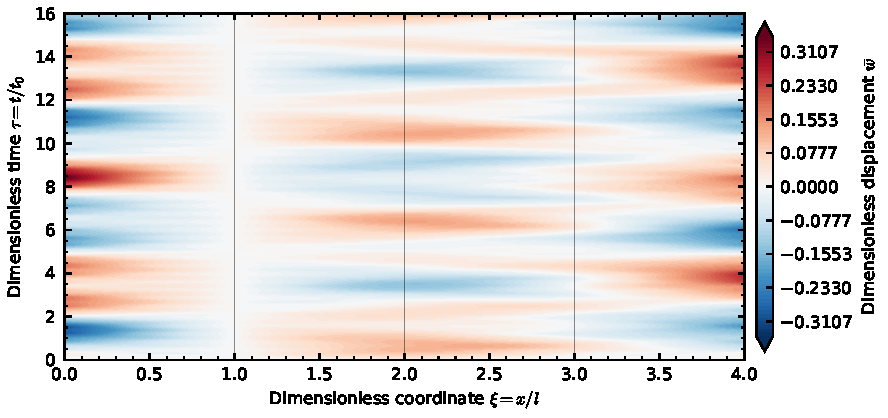
\includegraphics[width=\linewidth]{q3_spacetime_response.pdf}
    \column{0.32\linewidth}
    \small
    \begin{itemize}
      \item 横轴 $\xi=x/l$，纵轴 $\tau=t/t_0$，颜色为 $\bar{w}$
      \item 红色/蓝色区域交替：位移随时间的正负振荡
      \item $\xi=1$（$B$ 点支承）：位移始终为零，形成节线
      \item $\xi=2$（$C$ 点质量）：颜色过渡平滑，无突变
      \item $\xi=3$（$D$ 点弹簧）：振幅略微收窄，局部约束效应
      \item 颜色带沿 $\tau$ 轴倾斜：波沿梁长传播的速度信息
    \end{itemize}
  \end{columns}
\end{frame}

% ====== 17. 有限元模型 ======
\begin{frame}{有限元模型}
  \begin{block}{二节点 Euler--Bernoulli Hermite 梁单元}
    每节点两个自由度：$\{w,\;\theta\}$
  \end{block}
  \vspace{0.3em}
  \begin{block}{单元刚度矩阵}
    \[
    \mathbf k_e=
    \frac{EJ}{h^3}
    \begin{bmatrix}
    12 & 6h & -12 & 6h\\[0.2em]
    6h & 4h^2 & -6h & 2h^2\\[0.2em]
    -12 & -6h & 12 & -6h\\[0.2em]
    6h & 2h^2 & -6h & 4h^2
    \end{bmatrix}
    \]
  \end{block}
\end{frame}

% ====== 18. 局部构件 FEM 处理 ======
\begin{frame}{局部构件的有限元处理}
  \begin{columns}[T,onlytextwidth]
    \column{0.50\linewidth}
    \begin{itemize}
      \item $B$ 点：消元法施加 $w_B=0$，保留转角自由度
      \item $C$ 点：集中质量加入节点平动质量项
      \item $D$ 点：弹簧刚度加入节点平动刚度项
    \end{itemize}
    \column{0.46\linewidth}
    \begin{block}{广义特征值问题}
      \[
      \mathbf K\boldsymbol\Phi_n
      =
      \omega_n^2
      \mathbf M\boldsymbol\Phi_n
      \]
    \end{block}
  \end{columns}
  \vspace{0.6em}
  \begin{columns}[T,onlytextwidth]
    \column{0.50\linewidth}
    \begin{block}{离散参数}
      \begin{itemize}
        \item 单元数 $N_e=80$
        \item 节点数 $81$
      \end{itemize}
    \end{block}
    \column{0.46\linewidth}
    \begin{block}{响应叠加}
      前 $24$ 阶模态截断
    \end{block}
  \end{columns}
\end{frame}

% ====== 19. 程序流程 ======
\begin{frame}{程序与数据流程}
  \begin{center}
    \begin{tikzpicture}[
      node distance=1.2cm,
      every node/.style={
        draw, rounded corners, align=center,
        minimum width=2.8cm, minimum height=0.85cm,
        fill=softgray, draw=tjublue, thick
      }
    ]
      \node (f) {\textbf{Fortran}\\FEM 求解};
      \node[right=of f] (c) {\textbf{CSV}\\数据导出};
      \node[right=of c] (p) {\textbf{Python}\\后处理};
      \node[right=of p] (s) {\textbf{SciencePlots}\\可视化};
      \draw[->,>=stealth,thick,tjublue] (f) -- (c);
      \draw[->,>=stealth,thick,tjublue] (c) -- (p);
      \draw[->,>=stealth,thick,tjublue] (p) -- (s);
    \end{tikzpicture}
  \end{center}
  \vspace{0.8em}
  \begin{table}
    \centering
    \small
    \begin{tabular}{ll}
      \toprule
      输出文件 & 内容 \\
      \midrule
      \texttt{fem\_frequencies.csv} & 有限元固有频率 \\
      \texttt{fem\_modes.csv}       & 有限元振型 \\
      \texttt{fem\_c\_response.csv} & $C$ 点动力响应 \\
      \texttt{frequency\_comparison.csv} & 解析--FEM 频率对比表 \\
      \bottomrule
    \end{tabular}
  \end{table}
\end{frame}

% ====== 20. 频率对比 ======
\begin{frame}{固有频率对比}
  \begin{columns}[T,onlytextwidth]
    \column{0.62\linewidth}
    \centering
    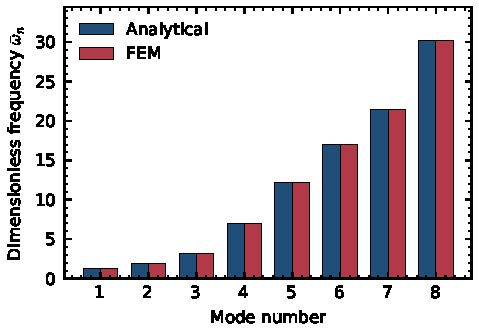
\includegraphics[width=\linewidth]{comparison_frequency_spectrum.pdf}
    \column{0.34\linewidth}
    \small
    \begin{itemize}
      \item Mode 1$\sim$8 柱状图中解析与 FEM 柱高肉眼不可分辨
      \item $\bar\omega_1\approx1.29$，$\bar\omega_8\approx30.2$，频率跨度约 23 倍
      \item 低阶频率增长较慢（Mode 1$\to$2 增量 $\approx0.66$）
      \item 高阶频率增速加快（Mode 7$\to$8 增量 $\approx8.76$）
      \item 趋势表明 FEM 空间离散对高阶影响开始显现
    \end{itemize}
  \end{columns}
\end{frame}

% ====== 21. 频率误差 ======
\begin{frame}{频率误差分析}
  \begin{columns}[T,onlytextwidth]
    \column{0.62\linewidth}
    \centering
    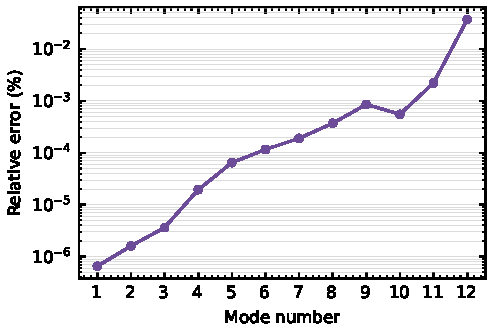
\includegraphics[width=\linewidth]{comparison_frequency_error.pdf}
    \column{0.34\linewidth}
    \small
    \begin{itemize}
      \item Mode 1 误差 $\approx6.6\times10^{-7}\%$，几乎为机器精度
      \item Mode 1$\sim$4 误差保持 $<2\times10^{-5}\%$
      \item Mode 5$\sim$11 误差从 $6.5\times10^{-5}\%$ 增至 $2.2\times10^{-3}\%$
      \item Mode 12 误差跳升至 $3.7\times10^{-2}\%$，发生质变
      \item 对数坐标下误差呈分段线性增长，转折点约在 Mode 11
    \end{itemize}
  \end{columns}
\end{frame}

% ====== 22. 振型对比 ======
\begin{frame}{振型对比}
  \begin{columns}[T,onlytextwidth]
    \column{0.66\linewidth}
    \centering
    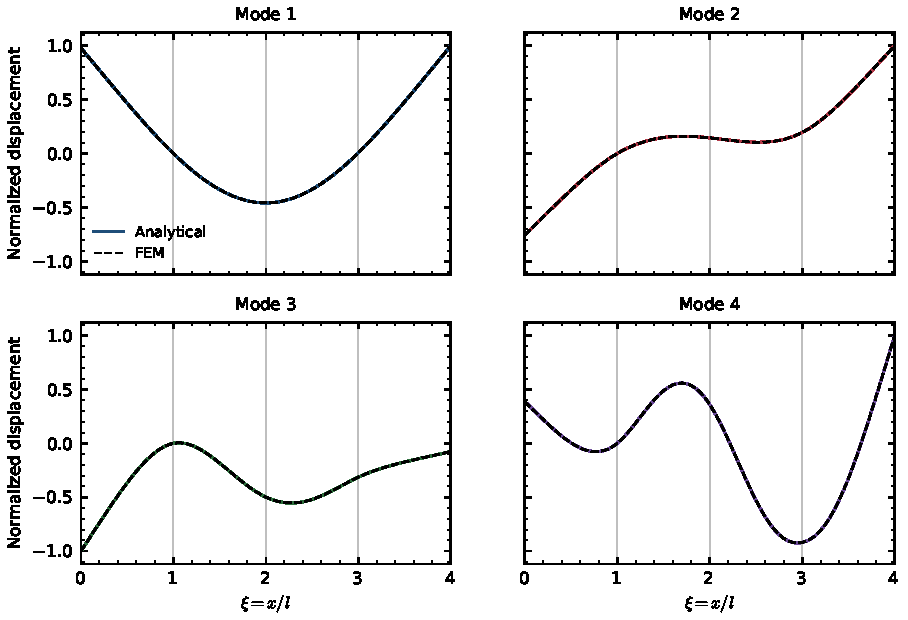
\includegraphics[width=\linewidth]{comparison_mode_overlay.pdf}
    \column{0.30\linewidth}
    \small
    \begin{itemize}
      \item 四子图逐一对比，FEM 虚线与解析实线完全叠合
      \item Mode 1 半波、Mode 2 单节线、Mode 3 双节线、Mode 4 三节线
      \item 节点位置、极值幅值均一致
    \end{itemize}
    \vspace{0.2em}
    \begin{block}{$L_2$ 相对误差}
      \[
      \begin{aligned}
      1:&\,2.455\times10^{-9}\\
      2:&\,1.727\times10^{-9}\\
      3:&\,2.404\times10^{-8}\\
      4:&\,5.903\times10^{-8}
      \end{aligned}
      \]
    \end{block}
  \end{columns}
\end{frame}

% ====== 23. 动力响应对比 ======
\begin{frame}{$C$ 点动力响应对比}
  \begin{columns}[T,onlytextwidth]
    \column{0.58\linewidth}
    \centering
    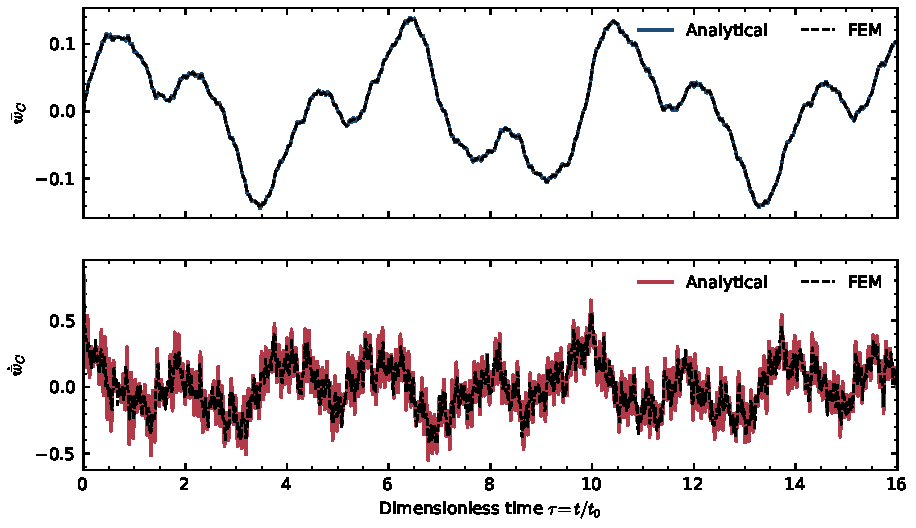
\includegraphics[width=0.95\linewidth]{comparison_c_response.pdf}
    \column{0.38\linewidth}
    \small
    \textbf{对比观察}
    \begin{itemize}
      \item 位移 $w_C$：解析（蓝实线）与 FEM（黑虚线）完全重合
      \item 速度 $\dot w_C$：模态叠加特征丰富，FEM 复现良好
      \item 位移 RMS 误差 $1.27\times10^{-3}$，速度 RMS 误差 $1.01\times10^{-1}$
      \item $\tau\to16$ 未见相位漂移，验证频率一致性
    \end{itemize}
  \end{columns}
\end{frame}

% ====== 24. 结论与展望 ======
\begin{frame}{结论与展望}
  \begin{columns}[T,onlytextwidth]
    \column{0.48\linewidth}
    \begin{block}{核心结论}
      \begin{enumerate}
        \item 传递矩阵法可有效处理集中质量和弹簧引起的状态跳跃
        \item 80 单元 FEM 模型准确复现前 11 阶固有频率与振型
        \item 动力响应对比中位移吻合极好，速度在低阶范围内一致
        \item 误差主要来自有限元空间离散和模态截断
      \end{enumerate}
    \end{block}
    \column{0.48\linewidth}
    \begin{block}{贡献总结}
      \begin{itemize}
        \item 解析解：为含离散构件的连续梁提供理论基准
        \item 数值解：FEM 配合传递矩阵法构成可扩展验证框架
        \item 工作流：Fortran 求解 + Python 后处理，完整可复现
      \end{itemize}
    \end{block}
  \end{columns}
  \vspace{0.6em}
  \begin{block}{展望}
    \small
    \begin{enumerate}
      \item 加密网格以提升高阶模态精度
      \item 研究不同 $\alpha$（质量比）和 $\kappa$（弹簧刚度）对频率和响应的影响规律
      \item 扩展至含阻尼、强迫振动、多点局部附件的更一般问题
    \end{enumerate}
  \end{block}
\end{frame}

\end{document}
